	\section{Introduction}

\subsection{Contexte}
\begin{frame}{Contexte}
Ces dernières années plusieurs catastrophes sont dues à des erreurs de spécifications des systèmes développés.
\begin{columns}
	\begin{column}{0.3\textwidth}
		\begin{figure}
			\begin{tikzpicture}		
				\only<1->
			{
				\node [inner sep=-10pt]
				{
					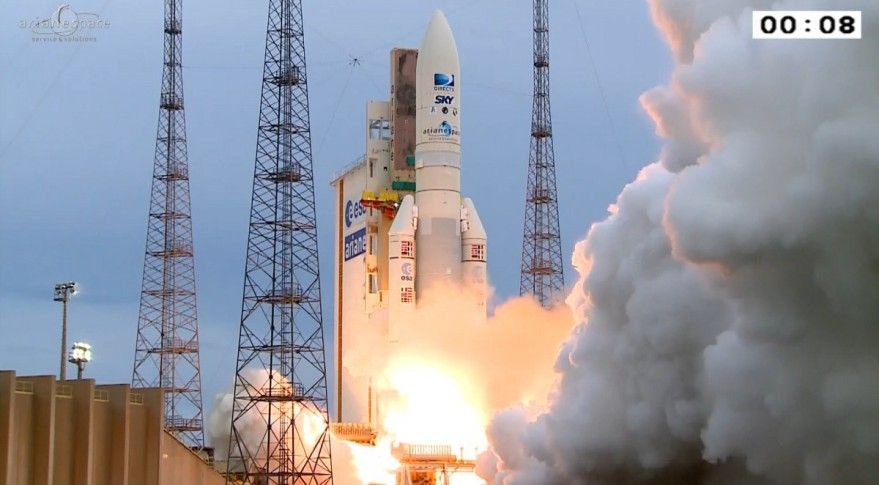
\includegraphics[height=1.2in,width=\columnwidth,trim={0 0 0 0},clip]{resources/Ariane_5}
				};              
			}
			\end{tikzpicture}
			\onslide<2->
			{  
				\caption{Ariane 5}
			}
		\end{figure}
	\end{column}

	\begin{column}{0.3\textwidth}
	\begin{figure}
		\begin{tikzpicture}		
		\only<3->
		{
			\node [inner sep=-10pt]
			{
				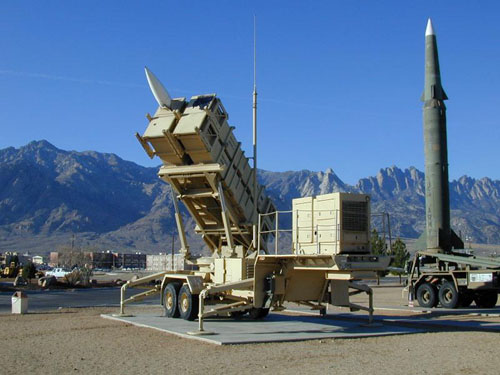
\includegraphics[height=1.2in,width=\columnwidth,trim={0 0 0 0},clip]{resources/Patriot}
			};              
		}
		\end{tikzpicture}
		\onslide<3->
		{  
			\caption{Missile Patriote}
		}
	\end{figure}
\end{column}

	\begin{column}{0.3\textwidth}
		\begin{figure}
			\begin{tikzpicture}
			\only<4->
			{
				\node [inner sep=-10pt]
				{
					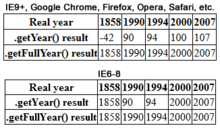
\includegraphics[height=1.2in,width=\columnwidth,trim={0 0 0 0},clip]{resources/bug2000}
				};
			}
			\end{tikzpicture} 
			\onslide<4->
			{
				\caption{Bug 2000}
			}
		\end{figure}
	\end{column}            
\end{columns}

\uncover<5->{%
La fiabilité de tout système est envisageable, en particulier celle de systèmes critiques.
}
%Vue l'importance de ces systèmes a complexité de ces systèmes il est pratiquement impossible de s'assurer que le système est fiable. 
\end{frame}

%La necessite d'utiliser les methodes formelle 
%les methodes formelle permet de prendre un systeme reel et la specifier formellement
\begin{frame}{}
\centering
\vspace{2.2cm}       
	\Huge 
		\textbf{Comment faire?}
%sachant que les jeux de test ne permet pas d'aboutir à une preuve contrainte
\end{frame}

\begin{frame}{titre section}
%le model checking permet de détecter automatiquement des erreurs dans le processus de
%conception, elle fournit aussi un contre-exemple en cas de non insatiabilité de la propriété dans le modèle permettant ainsi de corriger la source de l’erreur dans le
%système.

\begin{columns}[onlytextwidth,t]
	\column{.3\textwidth}
	\only<1->
	{
	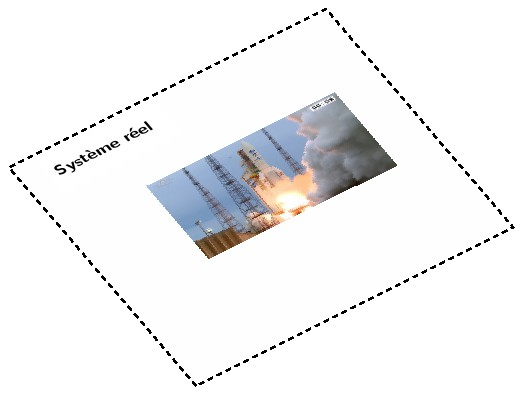
\includegraphics[height=1.2in,width=\columnwidth,clip=true,trim={-2 0 0 0}]{resources/mc/0001}
	}
	\column{.3\textwidth}
	\only<2->
	{
	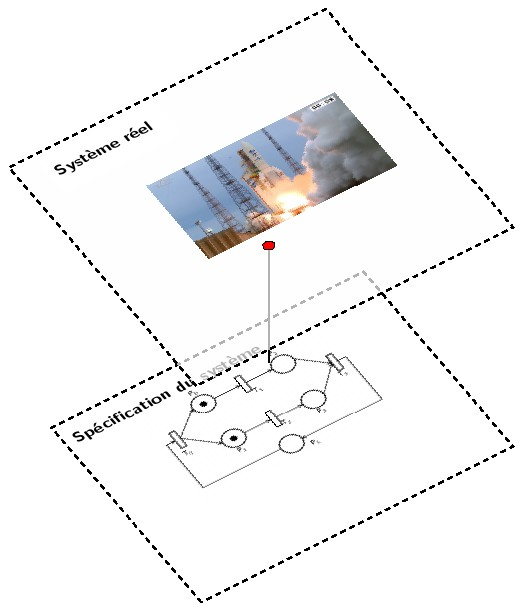
\includegraphics[height=1.2in,width=\columnwidth,clip=true,trim={0 0 0 0}]{resources/mc/0002}
	}
	\column{.3\textwidth}
	\only<3->
	{
	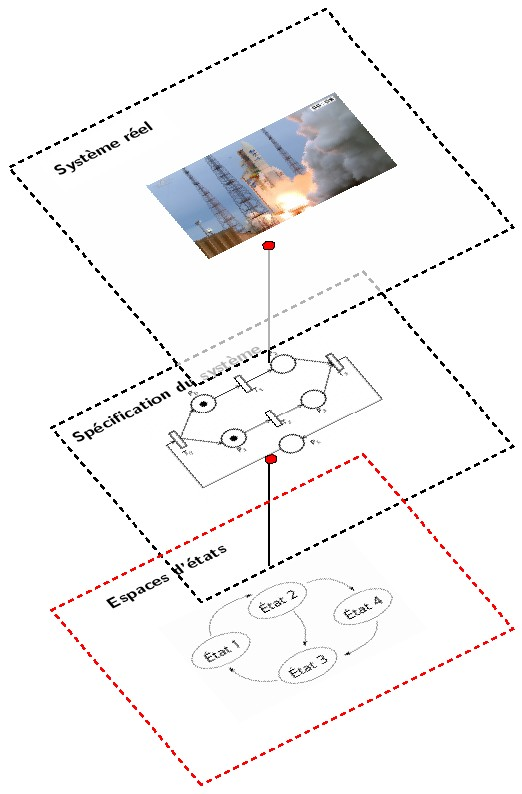
\includegraphics[height=1.2in,width=\columnwidth,clip=true,trim={0 0 0 0}]{resources/mc/0003}
	}
\end{columns}
\begin{columns}[onlytextwidth,t]
	\column{.3\textwidth}
	\only<4->
	{
		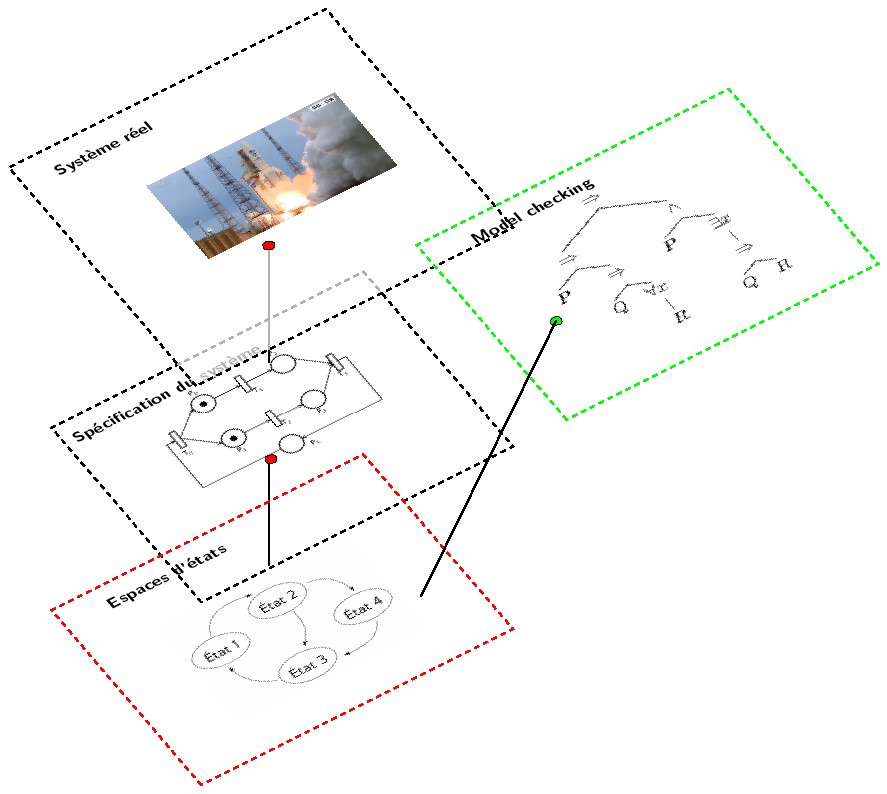
\includegraphics[height=1.2in,width=\columnwidth,clip=true,trim={0 0 0 0}]{resources/mc/0004}
	}
	\column{.3\textwidth}
	\only<5->
	{
		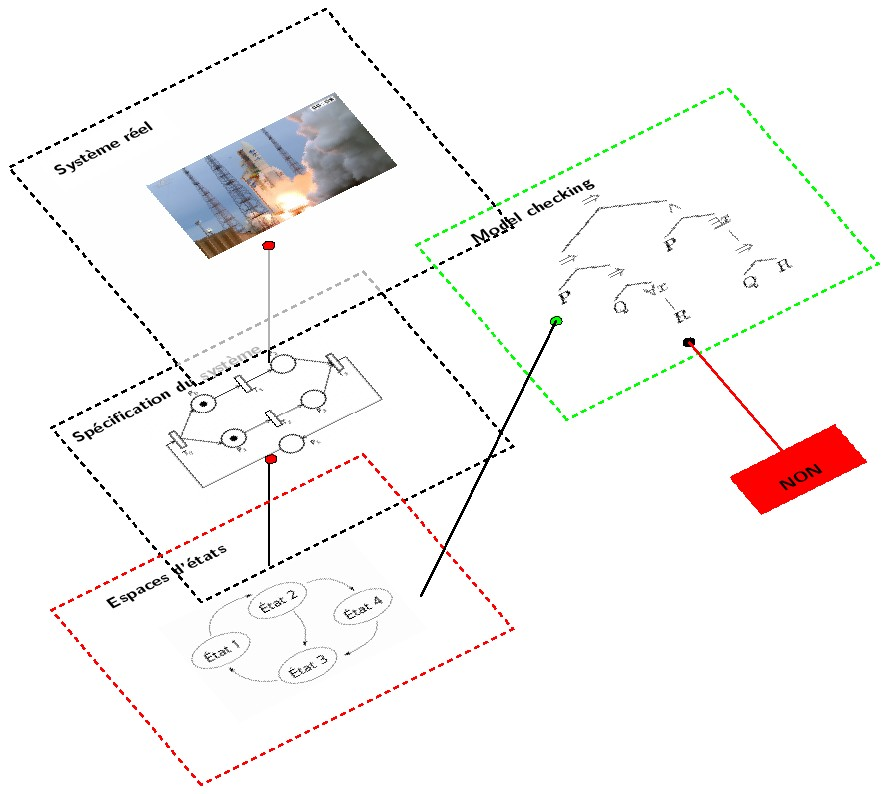
\includegraphics[height=1.2in,width=\columnwidth,clip=true,trim={0 0 0 0}]{resources/mc/0005}
	}
	\column{.3\textwidth}
	\only<6->
	{
		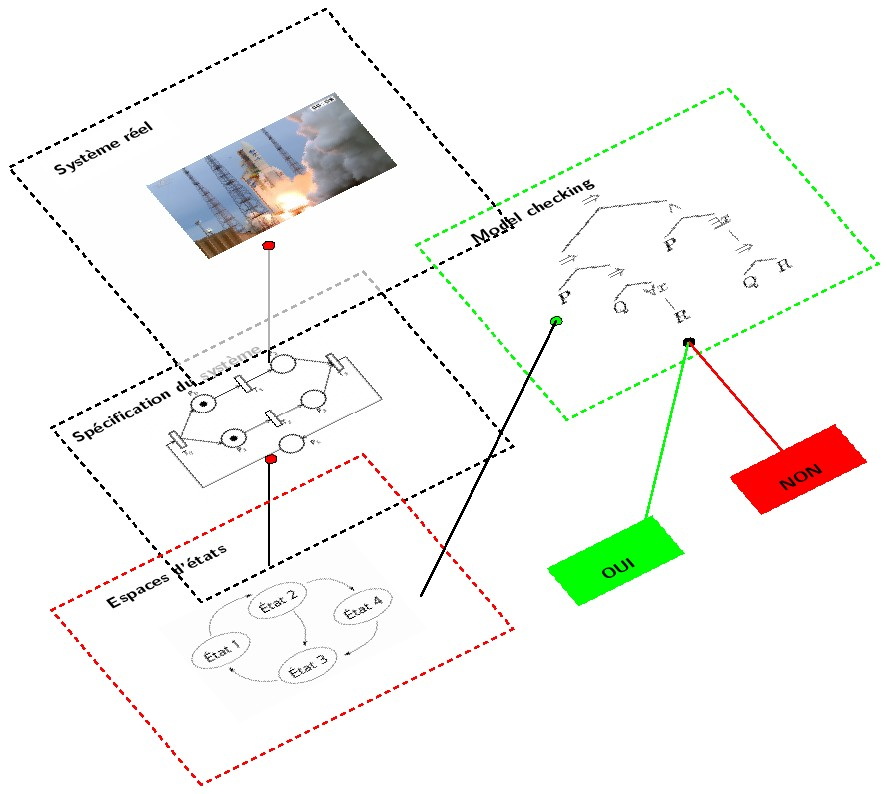
\includegraphics[height=1.2in,width=\columnwidth,clip=true,trim={0 0 0 0}]{resources/mc/0006}
	}
\end{columns}

\end{frame}

\begin{frame}
\centering
\vspace{2.2cm}       
\Huge 
\textbf{Problèmes}
%sachant que les jeux de test ne permet pas d'aboutir à une preuve contrainte
\end{frame}
\subsection{Problèmes}

\begin{frame}{titre section}

	\begin{center}
	 \begin{columns}
	 	\begin{column}{\textwidth}
	 		\begin{figure}
					% Define block styles
				\tikzstyle{decision} = [diamond, draw, fill=blue!20, 
				text width=4.5em, text badly centered, node distance=5cm, inner sep=0pt]
				\tikzstyle{block} = [rectangle, draw, fill=white, 
				text width=5em, text centered, rounded corners, minimum height=4em]
				\tikzstyle{line} = [draw, -latex']
				\tikzstyle{cloud} = [draw, ellipse,red!80, node distance=5cm,
				minimum height=2em]
				
				\begin{tikzpicture}[scale=3, every node/.style={scale=0.4},node distance = 5cm, auto]
				\only<2->
				{
					\node [decision ] (decide) {Peut-il être stocké sur une machine ?};
				}
				
				\node [cloud,fill=white,left of=decide] (g) {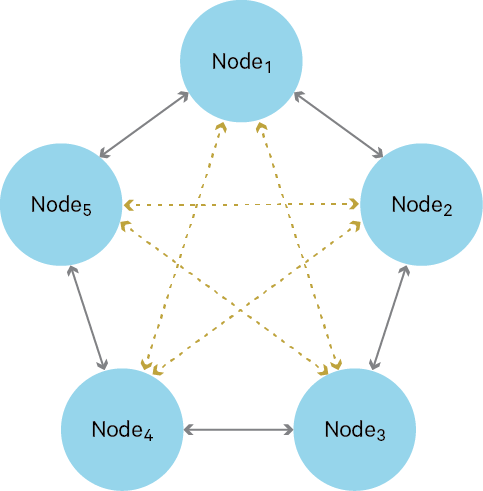
\includegraphics[width=1.5cm]{petri}};
				
				\only<3->
				{
					\node [block, below of=decide] (stockable) {
\includegraphics[width=1.5cm]{pc}};
				}
				\only<7->
				{
					\node [block, right of=decide,text width=10em, blue,node distance=10cm] (distribution)  {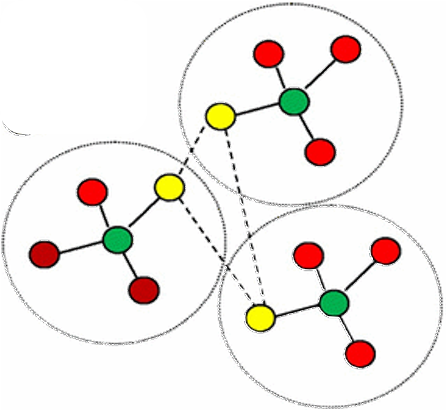
\includegraphics[width=3cm]{graphD}};
				}
				\only<5->
				{	
					\node [decision,below of=stockable] (tempsR) {Temps de reponse rainsonnable ?};
				}
				\only<6->
				{
					\node [block,left of=tempsR,blue ] (m) {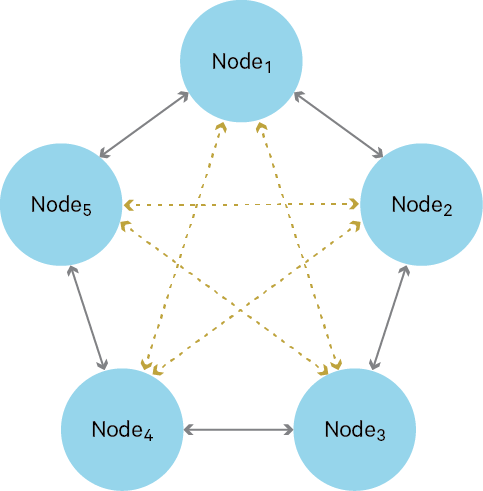
\includegraphics[width=2cm]{petri}};
				}
				\only<9->			
				{
					\node [block, right of=distribution,text width=10em,node distance=7cm ] (cdistribuer) {Comment Distribué ?}; 
				}
				% Draw edges
				\path [line,visible on=<2-> ] (g) -- (decide);
				\path [line,visible on=<3-> ] (decide) --node {OUI} (stockable);
				\path [line,visible on=<8-> ] (decide) -- node {NON}(distribution);
				\path [line,visible on=<5-> ] (stockable) --(tempsR);
				\path [line,visible on=<6-> ] (tempsR) -- node {OUI}(m);
				\path [line,visible on=<7-> ] (tempsR) -| node [near start] {NON}(distribution);
				\path [line,visible on=<9-> ] (distribution) -- (cdistribuer);
				
				\end{tikzpicture}

	 		\end{figure}
	 	\end{column}
 	\end{columns}
	\end{center}

\end{frame}


\begin{frame}
\centering
\vspace{2.2cm}       
\Huge 
\textbf{Comment distribué ?}
%chercher a surcharger une machine faira qu'augmenter le temps de la verification
\end{frame}

\subsection{Motivation}
\begin{frame}{Motivation}
\begin{columns}
	\begin{column}{0.4\textwidth}
		\begin{figure}	
			\only<1->
			{
			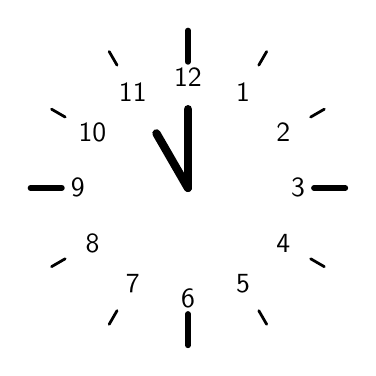
\begin{tikzpicture}[cap=round,line width=3pt]
		%	\filldraw [fill=examplefill] (0,0) circle (2cm);
			\foreach \angle / \label in
			{0/3, 30/2, 60/1, 90/12, 120/11, 150/10, 180/9,
				210/8, 240/7, 270/6, 300/5, 330/4}
			{
				\draw[line width=1pt] (\angle:1.8cm) -- (\angle:2cm);
				\draw (\angle:1.4cm) node{\textsf{\label}};
			}
			\foreach \angle in {0,90,180,270}
			\draw[line width=2pt] (\angle:1.6cm) -- (\angle:2cm);
			\draw (0,0) -- (120:0.8cm); % hour
			\draw (0,0) -- (90:1cm); % minute
			\end{tikzpicture}%         
			}
		
		\end{figure}
	\end{column}
	
	\begin{column}{0.4\textwidth}
		\begin{figure}
			\begin{tikzpicture}		
			\only<3->
			{
				\node [inner sep=-10pt]
				{
					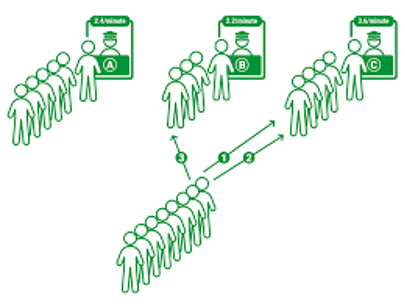
\includegraphics[width=\columnwidth,trim={0 0 0 0},clip]{resources/bndistributions}
				};              
			}
			\end{tikzpicture}			
		\end{figure}
	\end{column}   
\end{columns}


\end{frame}
